\documentclass[preview,varwidth]{standalone}
% basic math
\usepackage{physics,amsmath,amssymb}
\newcommand{\f}{\frac}
\newcommand{\p}[1]{\left(#1\right)}
\newcommand{\set}[1]{\left\{#1\right\}}

% color definitions (used in a figure)
\usepackage{xcolor}
\definecolor{orange}{RGB}{255,127,14}
\definecolor{green}{RGB}{44,160,44}

% proper coloring inside math environment
\makeatletter
\def\mathcolor#1#{\@mathcolor{#1}}
\def\@mathcolor#1#2#3{
  \protect\leavevmode
  \begingroup
    \color#1{#2}#3
  \endgroup
}
\makeatother

% particle diagrams
\usepackage{tikz}
\tikzset{
  baseline = (current bounding box.center)
}
\usetikzlibrary{math}
\usetikzlibrary{calc}
\usetikzlibrary{patterns}
\usetikzlibrary{decorations.pathmorphing}

\usepackage{braket}

\begin{document}
$
\vcenter{\hbox{
    \includegraphics[scale=0.55]{3LD_geometry.pdf}
  }}
\scalebox{0.9}{
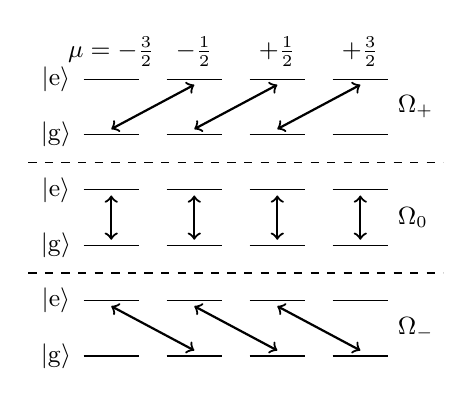
\begin{tikzpicture}
  %%% bottom
  \foreach \yy in {0em,2em} {
    \draw (0,\yy) -- (2em,\yy);
    \draw (3em,\yy) -- (5em,\yy);
    \draw (6em,\yy) -- (8em,\yy);
    \draw (9em,\yy) -- (11em,\yy);
  }
  \node () at (-1em,0) {\small$\ket{\mathrm{g}}$};
  \node () at (-1em,2em) {\small$\ket{\mathrm{e}}$};
  \node[right] () at (11em,1em) {\small$\Omega_-$};
  %
  \draw[<->,thick] (1em,1.8em) -- (4em,.2em);
  \draw[<->,thick] (4em,1.8em) -- (7em,.2em);
  \draw[<->,thick] (7em,1.8em) -- (10em,.2em);
  %%% middle
  \foreach \yy in {4em,6em} {
    \draw (0,\yy) -- (2em,\yy);
    \draw (3em,\yy) -- (5em,\yy);
    \draw (6em,\yy) -- (8em,\yy);
    \draw (9em,\yy) -- (11em,\yy);
  }
  \node () at (-1em,4em) {\small$\ket{\mathrm{g}}$};
  \node () at (-1em,6em) {\small$\ket{\mathrm{e}}$};
  \node[right] () at (11em,5em) {\small$\Omega_0$};
  %
  \draw[<->,thick] (1em,5.8em) -- (1em,4.2em);
  \draw[<->,thick] (4em,5.8em) -- (4em,4.2em);
  \draw[<->,thick] (7em,5.8em) -- (7em,4.2em);
  \draw[<->,thick] (10em,5.8em) -- (10em,4.2em);
  %%% top
  \foreach \yy in {8em,10em} {
    \draw (0,\yy) -- (2em,\yy);
    \draw (3em,\yy) -- (5em,\yy);
    \draw (6em,\yy) -- (8em,\yy);
    \draw (9em,\yy) -- (11em,\yy);
  }
  \node () at (-1em,8em) {\small$\ket{\mathrm{g}}$};
  \node () at (-1em,10em) {\small$\ket{\mathrm{e}}$};
  \node[right] () at (11em,9em) {\small$\Omega_+$};
  %
  \draw[<->,thick] (4em,9.8em) -- (1em,8.2em);
  \draw[<->,thick] (7em,9.8em) -- (4em,8.2em);
  \draw[<->,thick] (10em,9.8em) -- (7em,8.2em);
  %%% separating lines
  \foreach \yy in {3em,7em} {
    \draw[dashed] (-2em,\yy) -- (13em,\yy);
  }
  %%% nuclear spin labels
  \node() at (1em,11em) {\small$\mu=-\frac{3}{2}$};
  \node() at (4em,11em) {\small$-\frac{1}{2}$};
  \node() at (7em,11em) {\small$+\frac{1}{2}$};
  \node() at (10em,11em) {\small$+\frac{3}{2}$};
\end{tikzpicture}
}
$
\end{document}

%%% Local Variables:
%%% mode: latex
%%% TeX-master: t
%%% End:
